    \section{Rover}

    \subsection{Setup}
    For the setup process, we followed the tutorial from Freenove.
    The tutorial can be found here:
    \href{https://github.com/Freenove/Freenove_Three-wheeled_Smart_Car_Kit_for_Raspberry_Pi/blob/master/Tutorial.pdf}{\textbf{Three Wheeled Smart Car Kit for RPi - Tutorial}}.

    \subsubsection{Hardware Setup}

% --------- Block 1 ---------
    \noindent
    \begin{minipage}[t]{0.63\textwidth}
        \vspace*{0pt}
        The first step in the hardware setup was assembling the vehicle’s chassis. The acrylic chassis components had to be connected using plug connections, screws, and nuts. Since it was not possible to build the entire structure at once, we first created several subassemblies using the different acrylic parts.
    \end{minipage}
    \hfill
    \begin{minipage}[t]{0.33\textwidth}
        \vspace*{0pt}
        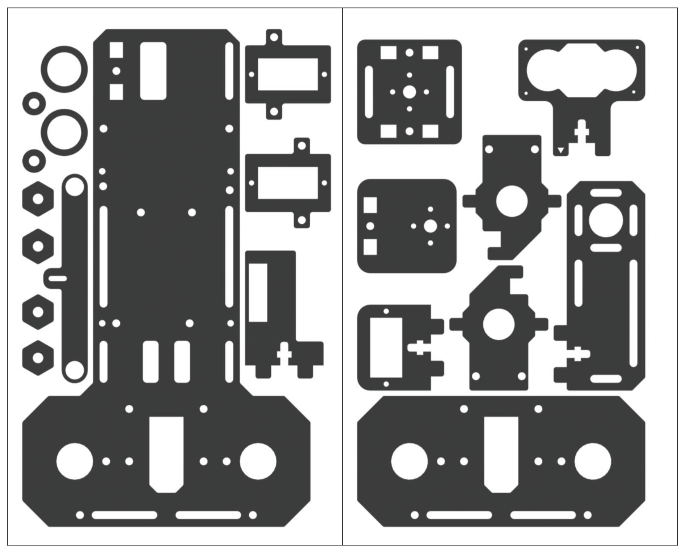
\includegraphics[width=\linewidth]{img/acrylic_sheets}
    \end{minipage}

    \vspace{1.5em}

% --------- Block 2 ---------
    \noindent
    \begin{minipage}[t]{0.63\textwidth}
        \vspace*{0pt}
        After preparing the main structural components, we mounted the servo motors and sensors onto the respective subassemblies. This required careful placement to ensure proper alignment and functionality.
    \end{minipage}
    \hfill
    \begin{minipage}[t]{0.33\textwidth}
        \vspace*{0pt}
        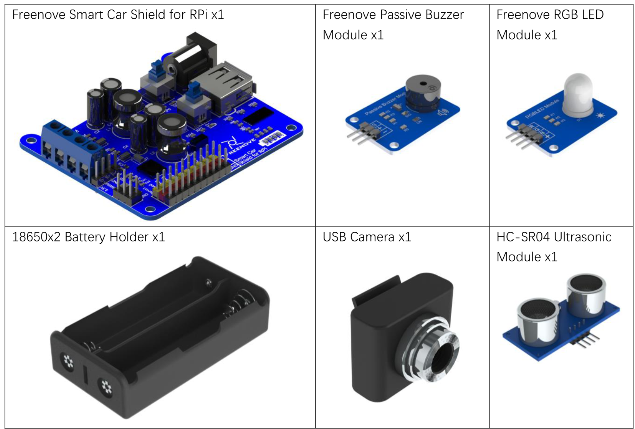
\includegraphics[width=\linewidth]{img/shield_and_sensors}
    \end{minipage}

    \vspace{1.5em}

% --------- Block 3 ---------
    \noindent
    \begin{minipage}[t]{0.63\textwidth}
        \vspace*{0pt}
        Once all parts were ready, we assembled the full vehicle by attaching the wheels and drive motors to the chassis. At this point, the main mechanical structure of the smart car was completed.
    \end{minipage}
    \hfill
    \begin{minipage}[t]{0.33\textwidth}
        \vspace*{0pt}
        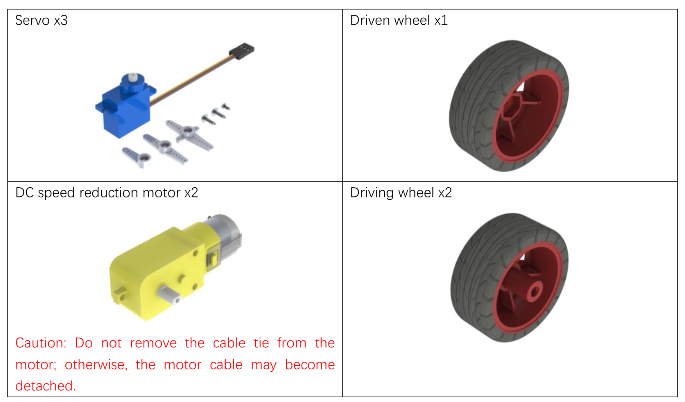
\includegraphics[width=\linewidth]{img/engine_and_wheels}
    \end{minipage}

    \vspace{1.5em}

% --------- Block 4 ---------
    \noindent
    \begin{minipage}[t]{0.63\textwidth}
        \vspace*{0pt}
        In the final step, we mounted the Raspberry Pi along with the included shield onto the chassis. We inserted the batteries into the holder and connected the motors, sensors, and other components to the shield using jumper cables.
    \end{minipage}
    \hfill
    \begin{minipage}[t]{0.33\textwidth}
        \vspace*{0pt}
        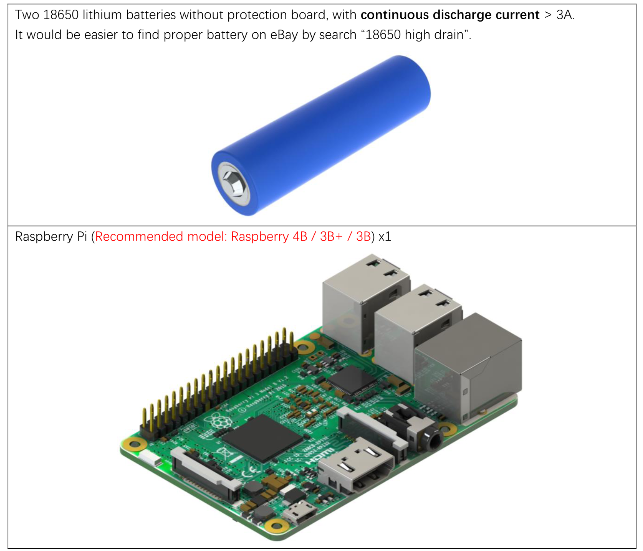
\includegraphics[width=\linewidth]{img/rpi_and_battery}
    \end{minipage}

    \vspace{1.5em}

% --------- Block 5 ---------
    \noindent
    \begin{minipage}[t]{0.63\textwidth}
        \vspace*{0pt}
        The cables of the individual components were connected to the Raspberry Pi shield according to the pinout shown in the image.
    \end{minipage}
    \hfill
    \begin{minipage}[t]{0.33\textwidth}
        \vspace*{0pt}
        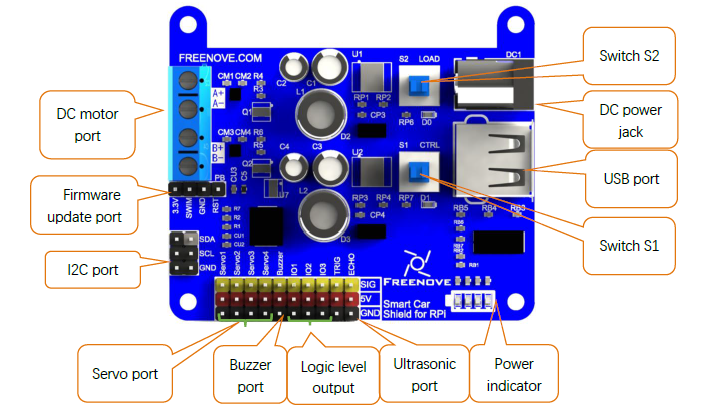
\includegraphics[width=\linewidth]{img/shield_pinout}
    \end{minipage}

    \vspace{2em}


    \subsubsection{Software Setup}

    First, we had to flash a micro SD card with an image compatible with the Raspberry Pi. We used the Raspbian Buster Full image and the Raspberry Pi Imager for this task.

    Once the image was ready, we powered up the Raspberry Pi and connected it to a temporary display. Then, we connected the Pi to our Wi-Fi hotspot and noted down its IP address to enable remote access via SSH or Remote VNC.

    Next, several settings had to be adjusted to allow remote connections:
    \begin{itemize}
        \item Enable I2C interface
        \item Enable VNC server
        \item Install XRDP
        \item Adjust screen resolution
    \end{itemize}

    Finally, we cloned the Git repository for testing purposes:
    \begin{verbatim}
git clone http://github.com/Freenove/Freenove_Three-wheeled_Smart_Car_Kit_for_Raspberry_Pi.git
    \end{verbatim}

    Additionally, we installed several required packages:
    \begin{itemize}
        \item i2c-tools
        \item python-smbus
    \end{itemize}

    After this steps, we were able to connect to the RPi remotely.

    \subsubsection{Testing}
    After preparing both the hardware and software, we tested the individual servo motors and the drive motors to check if they were working properly.

    For this purpose, we used pre-made test scripts from the cloned Git repository:
    \begin{verbatim}
        python mDev.py servo
        python mDev.py buzzer
        python mDev.py motor
        python mDev.py RGBLED
    \end{verbatim}

    Once we confirmed that everything was functioning correctly, we could focus on developing our own software.

    \subsection{Software}

    The software in the \texttt{rover/} folder controls the PiRover's hardware and manages communication between the Raspberry Pi and the web interface. Below is a short explanation of each file and how they work together.

    The file \texttt{main.py} is the starting point of the system. It uses functions from \texttt{hardware.py} to control motors and LEDs, uses \texttt{camera.py} to get live video, and starts communication via \texttt{mqtt.py} and \texttt{websocket.py}.
    The modules are connected like this:
    \begin{itemize}
        \item \texttt{main.py} imports and coordinates all other modules.
        \item \texttt{hardware.py} is used by \texttt{main.py} and \texttt{test.py} to control the hardware.
        \item \texttt{camera.py} is used by \texttt{main.py} to send video frames.
        \item \texttt{mqtt.py} and \texttt{websocket.py} handle communication, both started from \texttt{main.py}.
        \item \texttt{util.py} is a helper used by \texttt{hardware.py} for scaling values.
        \item \texttt{test.py} tests \texttt{hardware.py}.
    \end{itemize}

    \subsubsection*{\texttt{main.py}}
    This is the main program. It:
    \begin{itemize}
        \item resets the hardware,
        \item starts the WebSocket server,
        \item connects to the MQTT broker.
    \end{itemize}
    It also sends commands to the hardware and streams live camera feed.

    \subsubsection*{\texttt{hardware.py}}
    Controls the physical components using I2C:
    \begin{itemize}
        \item motors (driving and steering),
        \item camera servos,
        \item RGB LEDs,
        \item buzzer.
    \end{itemize}
    It includes a \texttt{reset()} function to stop all parts safely.

    \subsubsection*{\texttt{camera.py}}
    Uses OpenCV to read video frames from the camera. The frames are sent to the web interface as Base64-encoded JPEG images.

    \subsubsection*{\texttt{mqtt.py}}
    Handles MQTT communication. It connects to the MQTT broker, subscribes to topics, and sends or receives messages.

    \subsubsection*{\texttt{websocket.py}}
    Starts a WebSocket server for real-time communication with the frontend. It runs in a background thread.

    \subsubsection*{\texttt{util.py}}
    Contains a helper function \texttt{scale()} to convert values (e.g., servo angles or motor speed) into the correct format for I2C.

    \subsubsection*{\texttt{test.py}}
    Used to test the hardware components. It includes test functions for:
    \begin{itemize}
        \item servo motors,
        \item drive motors,
        \item RGB LEDs,
        \item the buzzer.
    \end{itemize}
    All parts are tested one after another.
